\chapter{Sound Source Separation \& \library{Separake}}\label{chap:separake}

\marginpar{%
    \footnotesize
    \textbf{Keywords:} Blind Channel Identification, Super Resolution, Sparsity, Acoustic Impulse Response.
    \\\textbf{Resources:}
    \begin{itemize}
        \item \href{https://doi.org/10.1109/ICASSP.2018.8461345}{Paper}
        \item \href{https://github.com/fakufaku/separake}{Code}
        \item \href{https://sigport.org/documents/separake-source-separation-little-help-echoes}{Slides}
    \end{itemize}
}
\newthought{Synopsis} \synopsisChSeparake

\mynewline
The material presented in the chapter results from a collaboration with Robin Scheibler and Ivan Dokmani\'{c} and wa published in~\cite{scheibler2018separake}.
This chapter recalls the main findings of the paper and brings additional insights on the literature and on the proposed model, which has been re-written using this thesis' notations.
The personal contribution to this collaboration, done in the early months of the \PhD/, was the implementation in Python of the proposed \EMdef/-\NMF/ method accounting for echoes and using a pre-trained dictionary.

\section{Literature review in Echo-aware Audio Source Separation}

%%%% rewrite it ######################### #TODO: rewrite this section accoring to Antoines comments
The scientific literature on audio source separation is vast, still active, and spans decades.
The problem covers a huge number of scenario and use-cases, such as number of microphones (single- \vs/ multi-channel recordings),
number of sources with respect to the number of channels (under- \vs/ over- \vs/ determined),
type of observed signals (speech \vs/ music), type of recordings (artificial \vs/ microphone recordings) \etc/, and, of course, combination of them.
In this chapter we will consider only the case of multichannel microphone recordings featuring reverberant speech data in overdetermined settings.
Even selecting this narrow case, the literature remain vast and we will not review it in the context of this thesis.
Instead, we will focus on multichannel source separation based on \acf{NMF}.
\ac{NMF} refers to a set of technique to model spectra of complex sounds by a sum of basic components.
Modeling sound structure is beneficial for source separation, since it make separation possible in many challenging scenario.
Moreover, this approach allows to easily incorporate side information on both the sources and the acoustic propagation as will be shown later in the chapter.

Currently, in the literature, only few works can be found that incorporate the knowledge of echoes into sound source separation.
In the work \citeonly{huang2005blind}, the authors proposes a decomposition of the source separation problem into different steps.
First they estimate the \RIRs/ by extending the \SIMO/-\BCE/ framework form \MIMO/ systems.
Here the \RIRs/ are modeled as \FIR/ filters following the multipath echo model.
Secondly, the estimated filters are used to build the demixing matrix, and then to separate the sources with an inverse-filtering approach.
However, this method exhibits an high computational cost, which was addressed later in~\citeonly{rotili2010joint}.
Nevertheless these approaches were shown to lack robustness in low SNR conditions.
\\Alternatively, the work in~\citeonly{asaei2014structured} proposes an geometry-based approach embedded in a sparse optimization framework.
First, by localizing the image sources and estimating the room geometry, the supports of the \RIRs/' early contributions are estimated.
Then, after computing the coefficient of the \RIRs/ element in a convex optimization framework, the individual speech signals are separated with either inverse-filtering or sparse recovery.
The performance of this approach relies on the \RIR/ and geometry estimation steps, which are very sensitive to the challenging acoustic condition, \eg/ low SNR or high \RT.
\\Instead, the work in \citeonly{leglaive2015multichannel} proposes to tackle the convolutive model by imposing a probabilistic prior on the early part of the \RIRs/, namely, modeled as an autoregressive process in the frequency domain.
Later, the same authors extended this work in~\citeonly{leglaive2016multichannel} accounting for both early and late part of the mixing filters.


\newthought{The proposed approach} is yet different from those presented above.
First, rather than fitting the echo model as in~\citeonly{leglaive2015multichannel,leglaive2016multichannel}, or estimating the mixing filters as in~\citeonly{huang2005blind,asaei2014structured},
we aim to show that separation in the presence of known echoes is better than separation without echoes .
Second, we conduct this investigation in the context of source separation with non-negative source models.
Third, we propose to solve the problem from the point of view of \textit{image microphones}.
The image microphone model is equivalent to the \ISMdef/~\citeonly{allen1979image}, where virtual receivers are placed outside of the room (See~\cref{fig:separake:setup}).
Even if the \ISM/ is more common and implemented in practice in acoustic simulators, the two models are strictly equivalent.
Therefore, this is a reasonable model for early echoes when strongly reflective, non-diffuses surfaces are present near the sources and microphones, which commonly happens in a living room or conference room.
However, it incurs a significant mismatch with respect to the complete reverberation (See~\cref{ch:acoustics}).
This approach is based on the acoustic rake receivers previously proposed in~\citeonly{Dokmanic:2015dr} and is thus dubbed \SEPARAKEdef/.

\mynewline
The considered setup is illustrated in~\cref{fig:separake:setup}.
We assume that the array is placed close to a wall or a corner. This is useful for the following reasons.
First, it makes echoes from the nearby walls significantly stronger than all other echoes.
Second, it ensures that the resulting image array (real and image microphones) is compact, allowing to assume the far field regime.

\begin{figure}[t]
    \begin{sidecaption}[Separake setup]{%
        Typical setup with two speakers recorded by two microphones.
        The illustration shows the virtual microphone model (grey microphones) with direct sound path (dotted lines) and resulting first-order echoes (colored lines).
        \\Image taken from the paper~\citeonly{scheibler2018separake}.
        }[fig:separake:setup]
    \centering
    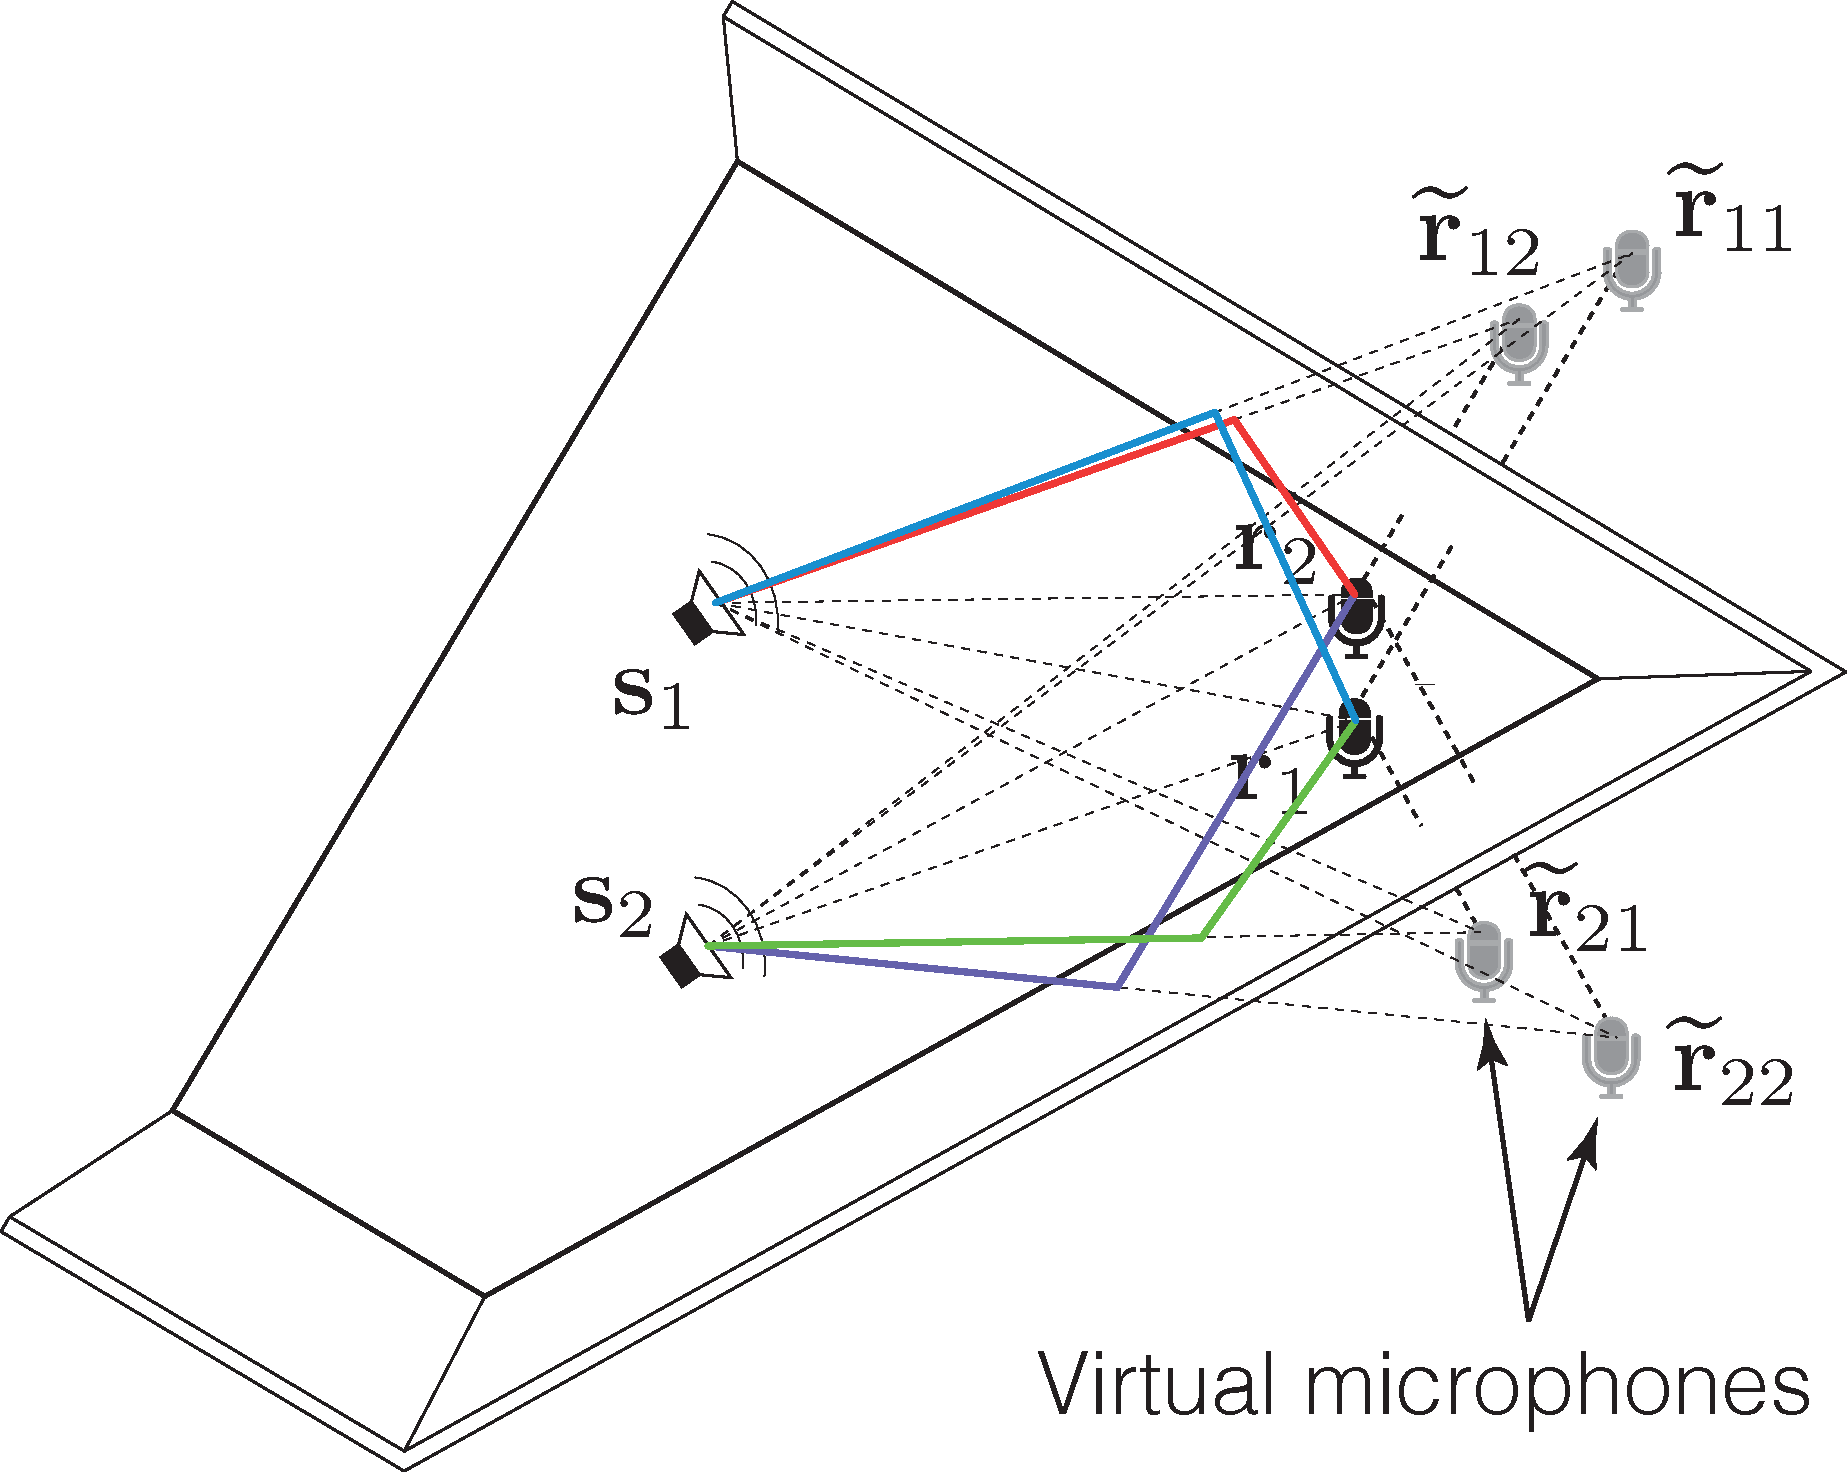
\includegraphics[width=.6\linewidth]{separake/separake.pdf}
    \end{sidecaption}
\end{figure}

\newthought{Translating echoes into image arrays} provides an interesting geometrical interpretation in light of beamforming theory.
Real and virtual microphones form dipoles with diverse frequency-dependent directivity patterns.
By integrating more and more virtual microphones, the directivity patterns change and higher spatial selectivity can be achieved~\citeonly{dokmanic2015raking}.
This effect is shown in~\cref{fig:separake:directivity}.
Therefore, the goal of this work is to design audio source separation algorithms which benefit from this known spatial diversity.
\begin{figure}[t]
    \begin{fullwidth}
    \centering
    \resizebox{\linewidth}{!}{
        

\tikzset{every picture/.style={line width=0.75pt}} %set default line width to 0.75pt

\begin{tikzpicture}[x=0.75pt,y=0.75pt,yscale=-1,xscale=1]
%uncomment if require: \path (0,300); %set diagram left start at 0, and has height of 300

%Image [id:dp3129430507137261]
\draw (100,148) node  {
\includegraphics[width=12pt]{acoustics/iconfinder_microphone_1608550.pdf}};
%Shape: Rectangle [id:dp30560892412693785]
\draw  [draw opacity=0][fill={rgb, 255:red, 255; green, 255; blue, 255 }  ,fill opacity=1 ] (30,40) -- (90,40) -- (90,100) -- (30,100) -- cycle ;
%Image [id:dp7096994311262355]
\draw (60,70) node  {
\includegraphics[width=45pt,height=45pt]{acoustics/iconfinder_ic_speaker_48px_352138.pdf}};

%Shape: Rectangle [id:dp4697494152917967]
\draw  [draw opacity=0][fill={rgb, 255:red, 155; green, 155; blue, 155 }  ,fill opacity=1 ] (120,20) -- (130,20) -- (130,180) -- (120,180) -- cycle ;
%Shape: Rectangle [id:dp004047242901594306]
\draw  [draw opacity=0][fill={rgb, 255:red, 155; green, 155; blue, 155 }  ,fill opacity=1 ] (30,170) -- (130,170) -- (130,180) -- (30,180) -- cycle ;
%Straight Lines [id:da07895276576528787]
\draw    (30,170) -- (120,170) -- (120,20) ;
%Image [id:dp41187969901424026]
\draw (150,148) node  {
\includegraphics[width=12pt]{acoustics/iconfinder_microphone_1608550.pdf}};
%Image [id:dp5789764730979481]
\draw (460,148) node  {
\includegraphics[width=12pt]{acoustics/iconfinder_microphone_1608550.pdf}};
%Shape: Rectangle [id:dp9000181446128821]
\draw  [draw opacity=0][fill={rgb, 255:red, 255; green, 255; blue, 255 }  ,fill opacity=1 ] (390,40) -- (450,40) -- (450,100) -- (390,100) -- cycle ;
%Image [id:dp2435207414441274]
\draw (420,70) node  {
\includegraphics[width=45pt,height=45pt]{acoustics/iconfinder_ic_speaker_48px_352138.pdf}};

%Shape: Rectangle [id:dp9398764926641255]
\draw  [draw opacity=0][fill={rgb, 255:red, 155; green, 155; blue, 155 }  ,fill opacity=1 ] (480,20) -- (490,20) -- (490,180) -- (480,180) -- cycle ;
%Shape: Rectangle [id:dp778971808734305]
\draw  [draw opacity=0][fill={rgb, 255:red, 155; green, 155; blue, 155 }  ,fill opacity=1 ] (390,170) -- (490,170) -- (490,180) -- (390,180) -- cycle ;
%Straight Lines [id:da3135305596380903]
\draw    (390,170) -- (480,170) -- (480,20) ;
%Image [id:dp7510496534085151]
\draw (510,148) node  {
\includegraphics[width=12pt]{acoustics/iconfinder_microphone_1608550.pdf}};
%Image [id:dp46570823643682746]
\draw (460,198) node  {
\includegraphics[width=12pt]{acoustics/iconfinder_microphone_1608550.pdf}};
%Shape: Rectangle [id:dp7037413163827391]
\draw  [draw opacity=0][fill={rgb, 255:red, 255; green, 255; blue, 255 }  ,fill opacity=0.69 ] (140,130) -- (160,130) -- (160,160) -- (140,160) -- cycle ;
%Shape: Rectangle [id:dp9860539015068507]
\draw  [draw opacity=0][fill={rgb, 255:red, 255; green, 255; blue, 255 }  ,fill opacity=0.69 ] (500,130) -- (520,130) -- (520,160) -- (500,160) -- cycle ;
%Shape: Rectangle [id:dp6314384514574135]
\draw  [draw opacity=0][fill={rgb, 255:red, 255; green, 255; blue, 255 }  ,fill opacity=0.69 ] (450,180) -- (470,180) -- (470,210) -- (450,210) -- cycle ;
%Image [id:dp35657556948669544]
\draw (250,100) node  {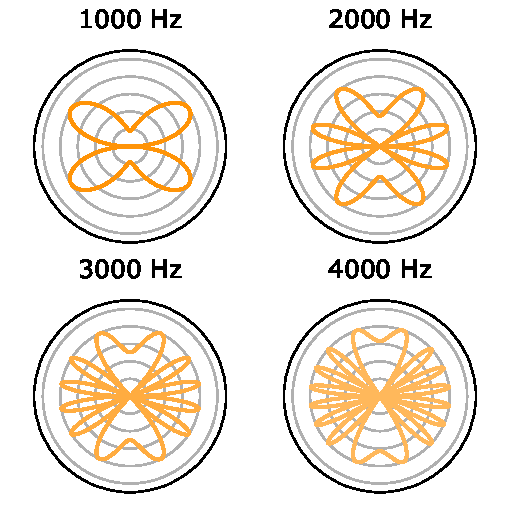
\includegraphics[width=120pt,height=120pt]{separake/rir_dipoles.pdf}};
%Image [id:dp09548352613616551]
\draw (610,100) node  {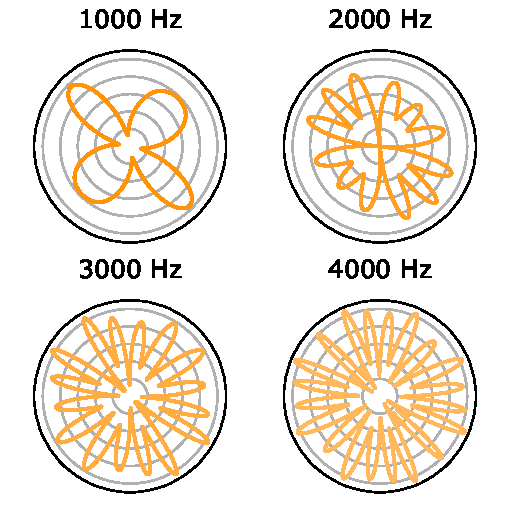
\includegraphics[width=120pt,height=120pt]{separake/rir_tripoles.pdf}};

% Text Node
\draw (105,212.5) node [anchor=north west][inner sep=0.75pt]  [font=\footnotesize] [align=left] {Virtual Dipoles};
% Text Node
\draw (472,212.5) node [anchor=north west][inner sep=0.75pt]  [font=\footnotesize] [align=left] {Virtual Tripoles};

\end{tikzpicture}

    }
    \label{fig:separake:directivity}
    \caption{The frequency-dependent directivity pattern for an virtual array built with a real and one (left) and two (right) image microphones.
    Image taken from }
    \end{fullwidth}
\end{figure}

\section{Modeling}
Recalling the echo model for the \RIRs/, and assuming $\numEchs$ echoes per source are known, the approximate \RTFdef/ from source $\idxSrc$ to microphone $\idxMic$ writes
\begin{equation}
    \label{eq:separake:approx_tf}
    \tilde{H}_{\idxMicSrc}(f) = \sum_{\idxEch=0}^{\numEchs} \alpha_{\idxMicSrc}^{(\idxEch)} \cste^{-\csti 2 \pi f \tau_{\idxMicSrc}^{(\idxEch)}}.
\end{equation}
Absolute  \acsp{TOA} relate to the source's distance which is not assumed to be known here.
Instead, we will assume that only the relative arrival times are known, by arbitrarily fix the delay of the direct path to zero.
This is equivalent to assume a far field scenario, thanks to which we can relate the relative \TOAs/ to the \DOAsdef/ of the source signal with respect to the center of the virtual array.
In addition, we assume all walls to be spectrally flat in the frequency range of interest and that $\alpha_{\idxMicSrc}^{(\idxEch)}$ are known up to a scaling (i.e. $\alpha_{\idxMicSrc}^{(0)} = 1$).
In this work the echoes properties are assumed to be known.

\mynewline
Assuming the narrowband approximation, the mixing process can be modeled as in \cref{subsec:processing:model:stft}.
Therefore, the \STFTdef/ of the $\idxMic$-th microphone signal reads
\begin{equation}
    \label{eq:separake:stft}
    \MIC_\idxMic[k,l] = \sum_{\idxSrc = 1}^{\numSrcs} H_{\idxMicSrc}[k] \SRC_{\idxSrc}[k,l] + \NSE_\idxMic[k,l]
\end{equation}
with $k\in\klist{0,\ldots,F}$ and $l\in\klist{0,\ldots,T}$ being the frequency and frame index,
$H_{\idxMicSrc}[k]$ is the \DFT/ approximating the \RTF/ of~\eqref{eq:separake:approx_tf},
$\MIC_{\idxSrc}[k,l]$ the \STFT/ of the $\idxSrc$-th source signal, and $\NSE_\idxMic[k,l]$ a term including noise and model mismatch.
It is convenient to group the microphone observations in vector-matrix form,
\begin{equation}
    \MICS[k,l] = \FLTSS[k]\SRCS[k,l] + \NSES[k,l]
    ,
\end{equation}
where $\MICS[k,l],  \NSES[k,l] \in \bbC^{\numMics \times 1}$, $\SRCS[k,l] \in \bbC^{\numSrcs \times 1}$ and $\FLTSS[k,l] \in \bbC^{\numMics \times \numSrcs}$.

\mynewline
Let the squared magnitude of the spectrogram of the $\idxSrc$-th source be $\mP_\idxSrc = \klist{\powerOf{\SRC_\idxSrc}}_{kl} \in \bbR^{F\times T}$.
As depicted in~\cref{fig:separake:nmf_source}, the spectrogram can be modeled as the product of 2 non-negative matrices:
\marginpar{
    \centering
    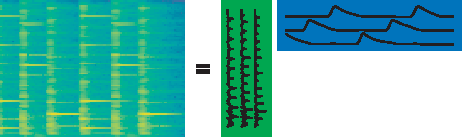
\includegraphics[width=\linewidth]{separake/nmf_example_source.pdf}
    \captionof{figure}{
        Spectrogram of a sound source signal decomposed into dictionary and activation.
        Image taken from the slides accompanying the paper of this work~\citeonly{scheibler2018separake}.
    }\label{fig:separake:nmf_source}
}
\begin{equation}
    \label{eq:separake:nmf}
    \mP_\idxSrc =  \mD_\idxSrc \mZ_\idxSrc,
\end{equation}
where $\mD_\idxSrc$ is the non-negative \textit{dictionary} whose columns are called \textit{atoms} and can be interpreted as interpreted as spectral templates of the source,
while the latent variables $\mZ_\idxSrc$, called \textit{activations}, indicating when and how this templates are activated.

\newthought{NMF-based Audio Source Separation} can then be cast as an inference problem in which we maximize the likelihood of the observed $\MICS$ over all possible non-negative factorizations \eqref{eq:separake:nmf}.
This normally involves learning the channels, namely the frequency-domain mixing matrices $\FLTSS$.
Instead of learning them, we build the channels based on the prior knowledge of the earliest few echoes.

\section{Source Separation by NMF}
In this work we consider two classical, well-understood multi-channel source separation algorithms which, by default, estimate the channels together with sources' dictionaries and activations.
The first algorithm is \NMFdef/ via \MUdef/ and consider only the magnitudes of the transfer functions.
The second one is the multichannel \NMF/ via \EMdef/, which instead explicitly models the phases of the mixing filters.
In this work, we considered only the (over)determined case ($\numSrcs \leq \numMics$).
In the following we briefly describe the idea behind the two algorithms.
We reminds to the work of~\citeonly{ozerov2010multichannel} for further details.

\subsection{NMF using Multiplicative Updates (MU-NMF)}\label{sec:separake:mu}
\MU/ for \NMF/ only involves the observed magnitude spectrograms only and the updates rules guarantee non-negativity as long as the initialization is non-negative.
This model has been originally proposed by in \citeonly{Lee:2001ti}, however we will consider its formulation as it appear in~\citeonly{ozerov2010multichannel}.
The observed multi-channel squared magnitude spectra are denoted $\mV_\idxMic = \klist{\powerOf{\MIC_\idxMic[k,l]}}_{kl}$ and their non-negative factorizations
\begin{equation}
    \label{eq:mu_nmf}
    \wh{\mV}_\idxMic = \sum_{\idxSrc=1}^{\numSrcs} \diag(\vQ_{\idxMicSrc}) \mD_\idxSrc \mZ_\idxSrc , \quad \idxMic=1,\ldots,\numMics
\end{equation}
\marginpar{
    \centering
    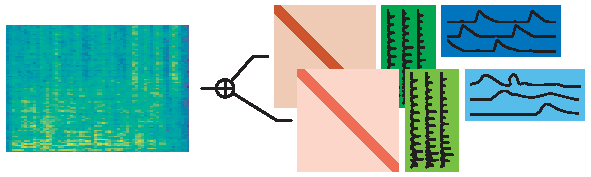
\includegraphics[width=\linewidth]{separake/mu_nmf_signal_model.pdf}
    \captionof{figure}{
        Schematics of the signal model used for \MU/-\NMF/.
    }\label{fig:separake:nmf_mu}
}
where $\vQ_{\idxMicSrc} = \klist{\powerOf{\FLT_{\idxMicSrc}[k]}}_k$ is the vector of squared magnitudes of the approximate \RTF/ between microphone $\idxMic$ and source $\idxSrc$.

\newthought{The MU rules minimize} the \textit{Itakura-Saito divergence} \citeonly{Fevotte:2011af} between the observed spectrogram $\mV_{\idxMic}[k,l]$ and the model $\wh{\mV}_{\idxMic}[k,l]$, that is, the cost function
\begin{equation}
    \scrC_{\mathtt{MU}}(\Theta_{\mathtt{MU}}) = \sum_{\idxSrc k l} \calD_{\mathtt{IS}}(\mV_{\idxMic}[k,l] | \wh{\mV}_{\idxMic}[k,l])
    + \gamma \sum_\idxSrc \kvvbar{\mZ_\idxSrc}_1,
\end{equation}
where $\calD_{\mathtt{IS}}( v | \hat{v} ) = \frac{v}{\hat{v}} - \log \frac{v}{\hat{v}} - 1$ and $\Theta_{\mathtt{MU}} = \{\vQ_{\idxMicSrc}, \set{\mD_\idxSrc, \mZ_\idxSrc}_\idxSrc\}_{\idxMicSrc}$ is the set of parameters.
We add an $\ell_1$-penalty term to promote sparsity in the activations due to the potentially large size of the dictionary~\citeonly{Sun:2013co}.

\newthought{The MU rule} for each scalar parameter of interest $\theta$ is obtained by multiplying its value at previous iteration by the ratio of the negative and positive parts of the derivative of the criterion \wrt/ this parameter, namely,
\begin{equation*}
    \theta \gets \theta \frac{\kbracket{\knabla_\theta \scrC_{\mathtt{MU}}(\Theta_{\mathtt{MU}})}_{-}}
                             {\kbracket{\knabla_\theta \scrC_{\mathtt{MU}}(\Theta_{\mathtt{MU}})}_{+}}
\end{equation*}
where $\scrC_{\mathtt{MU}}(\Theta_{\mathtt{MU}}) = {\kbracket{\knabla_\theta \scrC_{\mathtt{MU}}(\Theta_{\mathtt{MU}})}_{+}} - {\kbracket{\knabla_\theta \scrC_{\mathtt{MU}}(\Theta_{\mathtt{MU}})}_{-}}$ and the summands are both nonnegative.
Following the \MU/ rule derivations explained in \citeauthor{ozerov2010multichannel}, we obtain:
\begin{align}
    \vQ_{\idxMicSrc} &\gets\vQ_{\idxMicSrc} \odot \frac{\kbracket{\wh{\mV}_\idxSrc^{-2} \odot \mV_\idxSrc \odot \kparen{\mZ_\idxSrc \mD_\idxSrc}}\onesVect_{1\times T}}{
                                            \kbracket{\wh{\mV}_\idxSrc^{-1} \odot \kparen{\mZ_\idxSrc \mD_\idxSrc}}\onesVect_{1\times T}}\\
    \mZ_\idxSrc &\gets \mZ_\idxSrc \odot \frac{\sum_\idxMic \ktranspose{(\diag(\vQ_{\idxMicSrc}) \mD_\idxSrc)} \kparen{\mV_\idxSrc \odot \wh{\mV}_\idxSrc^{-2}}}{
                                            \sum_\idxMic \ktranspose{(\diag(\vQ_{\idxMicSrc}) \mD_\idxSrc)} \wh{\mV}_\idxSrc^{-1} + \gamma},\\
    \mD_\idxSrc &\gets \mD_\idxSrc \odot \frac{\sum_\idxMic \ktranspose{ \diag(\vQ_{\idxMicSrc})} \kparen{\mV_\idxSrc \odot \wh{\mV}_\idxSrc^{-2}}\ktranspose{\mZ_\idxSrc}}{
                                            \sum_\idxMic \ktranspose{ \diag(\vQ_{\idxMicSrc})} \wh{\mV}_\idxSrc^{-1} \ktranspose{\mZ_\idxSrc}},
\end{align}
where multiplication $\odot$, power, and division are element-wise and $\onesVect_{1\times T}$ is a $N$-vector of ones,.

\subsection{NMF using Expectation Maximization (EM-NMF)}\label{sec:separake:em}
Unlike the \MU/ algorithm that independently maximizes the log-likelihood of spectral magnitudes, the \EM/-\NMF/ maximizes the joint log-likelihood over all complex-valued channels~\citeonly{ozerov2010multichannel}.
Hence, the model takes explicitly into account observed phases.
In this approach, each source $\idxSrc$ is modeled as a complex Gaussian in the form of
\begin{equation}
    \SRC_\idxSrc[k,l] \sim \mathcal{N}_c \kparen{0, (\mD_\idxSrc\mZ_\idxSrc)_{kl}},
\end{equation}
and the magnitude spectrum $\mP_\idxSrc$ of \eqref{eq:separake:nmf} can be understood as the variance of source $\idxSrc$.
\\Under this model, and assuming uncorrelated noise, the microphone signals also follow a complex Gaussian distribution with covariance matrix
\begin{equation}
    \mSigma_{\MICS}[k,l] = \FLTSS[k] \mSigma_{\SRCS} [k,l] \khermitian{\FLTSS}[k] + \mSigma_{\NSES}[k,l]
    ,
\end{equation}
where $\mSigma_{\SRCS}$ and $\mSigma_{\NSES}$ are the covariance matrices of the sources and noise, respectively.

\newthought{The EM cost function} corresponds to the negative log-likelihood of the observed signal, that is,
\begin{equation}\label{eq:separake:loglike}
    \scrC_{\mathtt{EM}}(\Theta_{\mathtt{EM}}) = \sum\limits_{kl} \trace\kparen{\MICS[k,l] \khermitian{\MICS[k,l]} \mSigma_{\MICS}^{-1}[k,l]} \\
    + \log\det\mSigma_{\MICS}[k,l].
\end{equation}
where the $\Theta_{\mathtt{EM}} = \set{\FLTSS, \set{\mD_\idxSrc, \mZ_\idxSrc}_\idxSrc, \mSigma_{\NSES}}$ is the set of parameters.

\newthought{The EM algorithm} estimates all the parameters $\Theta$ by alternating between the so-called E-step and M-step.
In a nutshell, one iteration of the E-step consists in computing the \textit{conditional expectation} of the the ``complete'' log likelihood\sidenote{
    The complete data log-likelihood includes both observed variables $\MICS$ and latent variables $\SRCS$} with respect to the current parameter estimates,
and the M-step re-estimates the parameters by maximizing the conditional expectation of the complete log-likelihood.
This quantity can be efficiently minimized using the \EM/ algorithm proposed in~\citeonly{ozerov2010multichannel}.
Since adding sparsity priors is not straightforward in the \EM/ framework, it was not included in the proposed method.
% \begin{description}
%     \item[E-step:] Conditional expectation \wrt/ the current parameters
%     \begin{align}
%         a &= a\\
%         a &= a\\
%     \end{align}
%     \item[M-step:] Updates of the parameters
%     \begin{align}
%         \mD = \frac{1}{N} \sum_N
%     \end{align}
% \end{description}

% \subsection{Reconstruction of the sources}
% The reconstruction of the image sources is achieved by Wiener filtering, namely
% \begin{equation}
%     \IMG_\idxMicSrc[k,l] = \FLT_{\idxMicSrc}[k] \SRC_\idxSrc[k,l] =
% \end{equation}

\section{Echo-aware Source Separation}
To evaluate the usefulness of echoes in source separation, we modified the the multi-channel \NMF/ framework of \citeauthor{ozerov2010multichannel}~\citeonly{ozerov2010multichannel}.
The knowledge of the echoes is embedded in the model by approximating the entries of mixing matrices with~\eqref{eq:separake:approx_tf}, that is,
\begin{equation}
    \begin{aligned}
        \FLT_{\idxMicSrc}[k] &= \sum_{\idxEch=0}^{\numEchs} \alpha_{\idxMicSrc}^{(\idxEch)} \cste^{-\csti 2 \pi f_k \tau_{\idxMicSrc}^{(\idxEch)}},\\
        \FLTSS[k] &= \kbracket{\FLT_{\idxMicSrc}[k]}_{\idxMicSrc},
    \end{aligned}
\end{equation}
where $f_k = k\Fs/F$ are the discretized frequencies in Hz corresponding to the $k$-th bin in the \DFT/.
\\Futhermore, the early-echo channel model is kept fixed throughout the iterations.
Moreover, instead of updating both sources' dictionaries and activations, we adapted pre-trained dictionaries to better guide the source separation.

\newthought{Pre-trained Dictionaries} are a typical way to informing the \NMF/ algorithm, which is sometimes referred to as \textit{supervised \NMF/}.
The idea to run NMF on training sets containing examples from desired sound classes and collect the atoms of the estimated non-negative matrices\citeonly{schmidt2006single}.
At test phase, these atoms are used as basis vectors for the dictionary matrix (\ie/, $\mD$) and can be used as a good initialization point or kept fixed in the algorithm\sidenote{
    In the context of \NMF/-based music transcription applied to piano music, the dictionary can be a collection of spectral templates, each of which is associated to a piano note~\citeonly{muller2015fundamentals}}.
This can be seen as an instance of the problem of \textit{dictionary learning} which also exists in many other research fields.
For audio source separation, this idea has been studied extensively since promising results were obtained, even in single channel scenarios ~\citeonly{smaragdis2009sparse}.
As discussed later in~\cref{subsec:separake:dictionary}, in this work we will use two different dictionaries: one \textit{universal}, and the other \textit{speaker-specific}.

\newthought{Neglecting the reverberation} (or working in the anechoic regime) leads to a constant $\vQ_{\idxMicSrc}$ for all $\idxSrc$ and $\idxMic$.
A consequence is that the \MU/-\NMF/ framework breaks down with a unique, universal dictionary, namely, $\mD = \mD_j\;\forall j$.
Indeed, \eqref{eq:mu_nmf} becomes the same for all $\idxMic$,
\begin{equation*}
    \wh{\mV}_\idxMic = \sum_{\idxSrc} \mD \mZ_\idxSrc = \mD \sum_\idxSrc \mZ_\idxSrc,
\end{equation*}
so even with the correct atoms identified, we can assign them to any source without changing the value of the cost function.
Therefore, anechoic multi-channel separation with a universal dictionary cannot work well.
This intuitive reasoning is corroborated by numerical experiments in Section \ref{sec:results}.
The problem is overcome by the \EM/-\NMF/ algorithm which keeps the channel phase and is thus able to exploit the phase diversity across the array.
Of course, as showed in this work, it is also overcome by using echoes.

\section{Numerical Experiments}

We test our hypotheses through computer simulations.
In the following, we describe the simulation setup, dictionary learning protocols, and we discuss the results.

\subsection{Setup}
An array of three microphones arranged on the corners of an equilateral triangle with edge length $\SI{0.3}{\m}$ is placed in the corner of a 3D room with 7 walls.
We select 40 sources at random locations at a distance ranging from $\SI{2.5}{\m}$ to $\SI{4}{\m}$ from the microphone array.
Pairs of sources are chosen so that they are at least $\SI{1}{\m}$ apart.
The floor plan and the locations of microphones are depicted in Figure~\ref{fig:separake:rir_room}\marginpar{
    \centering
    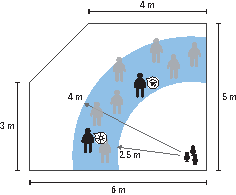
\includegraphics[width=\linewidth]{figures/separake/room_setup}
    \captionof{figure}{
        The simulated scenario.
        Image taken from the paper of this work~\citeonly{scheibler2018separake}
    }
    \label{fig:separake:rir_room}
}.
The scenario is repeated for every two active sources out of the 780 possible pairs.

\mynewline
The sound propagation between sources and microphones is simulated using the
image source model implemented in the \library{pyroomacoustics} Python package~\citeonly{scheibler2017pyroomacoustics}.
The wall absorption factor is set to $0.4$, leading to a $\RT$ of approximately $\SI{100}{\ms}$.
The sampling frequency is set to $\SI{16}{\kHz}$, \STFT/ frame size to $2048$ samples with $50\%$ overlap between frames, and we use a cosine window for analysis and synthesis.
Partial \RTFs/ are then built from the $\numEchs$ nearest image microphones.
The global delay is discarded, and only the relative amplitudes between echoes are kept.

\mynewline
With this setup, we perform three different experiments.
In the first one, we evaluate \MU/-\NMF/ with a universal dictionary.
In the other two, we evaluate the performance of \MU/-\NMF/ and \EM/-\NMF/ with speaker-specific dictionaries.
We vary $\numEchs$ from 1 to 6 and use the following three baseline scenarios:
\begin{enumerate}
\item \textit{anechoic}: Anechoic conditions, no model mismatch.
\item \textit{learn}: The \RTFs/ are learned from the data along the activations as originally proposed~\citeonly{ozerov2010multichannel} and the full reverberation is present in the observed data.
\item \textit{no echoes}: Reverberation is present but ignored (i.e. $\numEchs=0$).
\end{enumerate}
With the universal dictionary, the large number of latent variables warrants the introduction of sparsity-inducing regularization.
The value of the regularization parameter $\gamma$ was chosen by a grid search on a holdout set with the signal-to-distortion ratio ($\SDR$) as the figure of merit \citeonly{vincent2007first} (See ~\cref{tab:separake:gamma}).

\begin{table}
    \begin{sidecaption}[]{
        Value of the regularization parameter $\gamma$ used with the universal dictionary.
        }[tab:separake:gamma]
        \centering
        \small
        \begin{tabular*}{\linewidth}{@{\extracolsep{\fill}}lccccccccc@{}}
    \toprule
     &       &          & \multicolumn{7}{c}{{\footnotesize Number of echoes $\numEchs$}} \\
     \cmidrule{4-10}
     & anechoic & learn & 0 & 1 & 2 & 3 & 4 & 5 & 6 \\
     \cmidrule{2-10}
     $\gamma = $ & $10$ & $10^{-1}$ & $10$ & $10^{-3}$ & 0 & 0 & 0 & 0 & 0 \\
     \bottomrule
\end{tabular*}
    \end{sidecaption}
\end{table}


\subsection{Dictionary Training, Test Set}\label{subsec:separake:dictionary}
First, we introduce a dictionary learned from available training data.
We explore both speaker-specific and universal dictionaries \citeonly{Sun:2013co}.
Speaker-specific dictionaries can be beneficial when speakers are known in advance.
Universal dictionary is more versatile but gives a weaker regularization prior.
All dictionaries were trained on samples from the TIMIT corpus \citeonly{garofolo1993timit} using the \NMF/ solver in \library{scikit-learn} Python package~\citeonly{pedregosa2011scikit}.

\begin{figure}[h]
    \begin{fullwidth}
    \centering
    \subfloat[mu_univ][Universal dictionary]{
        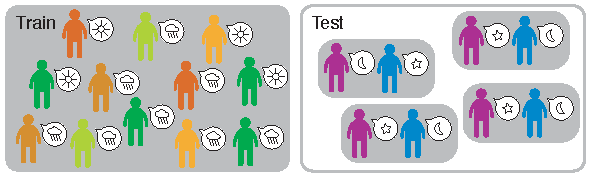
\includegraphics[width=0.48\linewidth]{separake/dict_universal.pdf}
        \label{fig:separake:dict_univ}}
    \hfill
    \subfloat[mu_spkr][Speaker-specific dictionary]{
        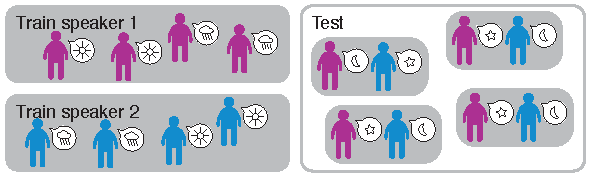
\includegraphics[width=0.48\linewidth]{separake/dict_speaker_dep.pdf}
        \label{fig:separake:dict_spk}}
        \caption{Schematic representation of the dictionary protocol used in this work.
        Image taken from the slides accompanying the paper of this work~\citeonly{scheibler2018separake}.}
    \label{fig:separake:results}
    \end{fullwidth}
\end{figure}


\newthought{Universal Dictionary:} Following the methodology of \citeonly{Sun:2013co} we select 25 male and 25 female speakers
and use all available training sentences to form the universal dictionary
$
    \mD = [\mD_1^\mathtt{M}\cdots \mD_{25}^\mathtt{M}\,\mD_{1}^\mathtt{F}\cdots\mD_{25}^\mathtt{F}].
$
The test signals were selected from speakers \emph{and} utterances outside the training set.
The number of latent variables per speaker is 10 so that with STFT frame size of 2048 we have $\mD\in\R^{1025\times500}$.

\newthought{Speaker-Specific Dictionary:}
Two dictionaries were trained on one male and one female speaker.
One utterance per speaker was excluded to be used for testing.
The number of latent variables per speaker was set to $20$.

\subsection{Implementation:}
Authors of \citeonly{ozerov2010multichannel} provide a Matlab implementation\sidenote{
    \href{http://www.irisa.fr/metiss/ozerov/Software/multi_nmf_toolbox.zip}{Multichannel nonnegative matrix factorization toolbox (in Matlab)}
} of \MU/-\NMF/ and \EM/-\NMF/ methods for stereo separation.
We ported their code to Python and extended it to arbitrary number of input channels\sidenote{
    In line with the philosophy of reproducible research, our implementation and all experimental code are publicly available at the \href{https://github.com/fakufaku/separake}{project repository}.
}.
However this software features some ad-hoc decisions which do not fit our scenario.
Thus, we provide a Python3 adaptation with the following modifications.
\begin{itemize}
    \item First the original code was restricted to the 2-channel case, i.e.  $\numMics = 2$.
    Thus, in order to embrace the specifics of our scenario and for the sake of generalization, we extend it to the multi-channel case, that is $\forall \numMics \geq 1$.
    \item the \MU/-\NMF/ was modified to handle sparsity constraint as described in \ref{sec:separake:mu}.
    \item since the \EM/ method degenerates when zero-valued entries are present in the dictionary matrix, $\mD$, all these entries are initially set to a small constant value of $10^{-6}$.
    \item the code was further modified to deal with fixed dictionary and channel models matrices, which are normalized in order to avoid indeterminacy issues \citeonly{ozerov2010multichannel}.
\end{itemize}
Finally, no \textit{simulated annealing} strategy was used in the final experiments.
In fact in some preliminary and informal investigations we noticed that this yielded better results than using annealing.
In the experiments, the number of iterations for \MU/-\NMF/ (\EM/-\NMF/) was set to $200$ ($300$).

\subsection{Results}
\label{sec:results}

We evaluate the performance in terms of signal-to-distortion ratio (\SDR) and source-to-interference ratio (\SIR) as defined in \citeonly{vincent2007first}.
We compute these metrics using the \library{mir\_eval} toolbox~\citeonly{raffel2014mir_eval}.

\mynewline
The distributions of \SDR{} and \SIR{} for separation using \MU/-\NMF/ and a universal dictionary are shown in \cref{fig:separake:mu_univ}, with a summary in \cref{fig:separake:median}.
We use the median performance to compare the results from different algorithms.
First, we confirm that separation fails for flat \RTFs/ (\textit{anechoic} and $\numEchs=0$) with \SIR{} at around 0~dB.
Learning the \RTFs/ performs somewhat better in terms of \SIR{} than in terms of \SDR{}, though both are low.
Introducing approximate \RTFs/ significantly improves performance: the proposed approach outperforms the learned approach even with a single echo.
With up to six echoes, gains are +2~dB \SDR{} and +5~dB \SIR{}.
Interestingly, with more than one echo, non-negativity and echo priors are already sufficient for achieving good separation, overtaking the $\ell_1$ regularization.


\begin{figure}[t]
    \begin{fullwidth}
    \centering
    \subfloat[mu_univ][MU-NMF, Universal dictionary]{
        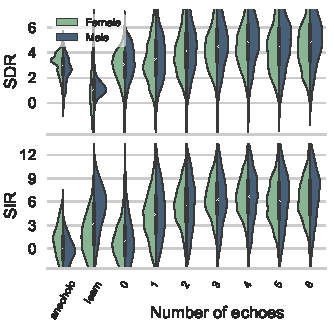
\includegraphics[width=0.32\linewidth]{separake/20171025-111558_5ae4058906_near_wall_mu_UnivDict_violin_plot.pdf}
        \label{fig:separake:mu_univ}}
    \hfill
    \subfloat[mu_spkr][MU-NMF, Speaker-specific dictionary]{
        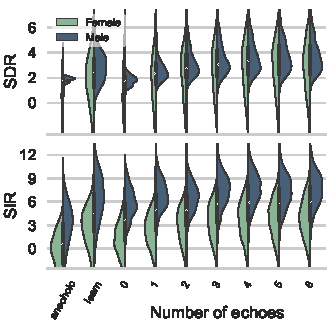
\includegraphics[width=0.32\linewidth]{separake/20171026-192746_360771b8ce_near_wall_mu_SpkrDict_violin_plot.pdf}
        \label{fig:separake:mu_spkr}}
    \hfill
    \subfloat[em_spkr][EM-NMF, Speaker-specific dictionary]{
        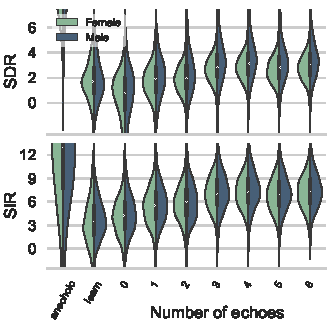
\includegraphics[width=0.32\linewidth]{separake/20171027-050909_e9d8c07aef6_near_wall_em_SpkrDict_violin_plot.pdf}
        \label{fig:separake:em_spkr}}
    \caption{Distribution of SDR and SIR for male and female speakers as a function of the number of echoes included in modeling, and comparison with the three baselines.}
    \label{fig:separake:results}
    \end{fullwidth}
\end{figure}


\begin{figure}[b]
    \begin{sidecaption}[]{
            Summary of the median SDR and SIR for the different algorithms evaluated.
            \label{fig:separake:median}
        }[fig:separake:median]
        \centering
        \small
        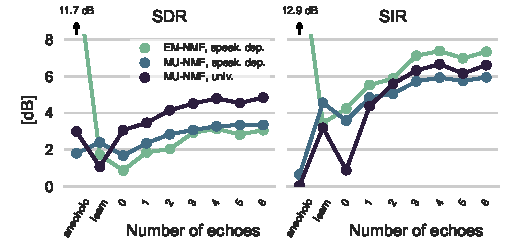
\includegraphics[width=\linewidth]{separake/all_medians.pdf}
    \end{sidecaption}
\end{figure}


\mynewline
Separation with speaker-dependent dictionaries is less challenging since we have a stronger prior.
Accordingly, as shown in ~\cref{fig:separake:mu_spkr,fig:separake:median}, \MU/-\NMF/ now achieves a certain degree of separation even without the channel information.
The gains from using echoes are smaller, though one echo is still sufficient to match the median performance of learned \RTFs/.
Using an echo, however, results in a smaller variance, while adding more echoes further improves \SDR{} (\SIR) by up to +2~dB (+3~dB).

\mynewline
In the same scenario, \EM/-\NMF/ (\cref{fig:separake:em_spkr}) has near-perfect performance on anechoic signals which is expected as the problem is overdetermined.
For \MU/, a single echo suffices to reach the performance of learned \RTFs/ and further improve it.
Moreover, echoes significantly improve separation quality as illustrated by up to 3~dB improvement over \textit{learn}.
It is interesting to note that in all experiments the first three echoes nearly saturate the metrics.
This is good news since higher order echoes are hard to estimate.

% \begin{itemize}
%    \item Universal dictionary scenario: Here, the speakers are unknown.
%    \begin{itemize}
%        \item Because the MU method does not use phase and hence no time delay information across channels, source separation in the anechoic scenario is impossible.
%              Here, we see that using reverberated signals instead with knowledge of only a few echoes significantly improve source separation performance: up to +2dB SDR and +5 dB SIR.
%        \item Using a fixed echo model for channels also outperform learning the channels, even with a single echo.
%        \item Note that EM could not be used for the universal dictionary scenario, because the corresponding model is not designed to handle dictionaries with hundreds of atoms. A sparsity-enforcing Bayesian prior on the estimated activation Z would need to be included, which is not straightforward.
%        \item Increasing the number of known echoes beyond 3 does not bring significant improvement.
%    \end{itemize}
%    \item Speaker-dependent dictionary scenario. This scenario is on the one hand easier because speakers are known and on the other hand harder because much less training data is used, allowing much fewer atoms to represent speech in the dictionaries.
%    \begin{itemize}
%        \item Unsurprisingly, EM performs extremely well in the anechoic setting. This is because perfect knowledge of the complex-valued over-determined mixing filters is then available, through the time differences of arrival. Results would likely be very different in an under-determined setting, where perfect filter knowledge is not enough to separate signals.
%        \item Once again, it is showed that using knowledge of a few echoes significantly improve results with respect to an anechoic model, up to +2dB SDR and +3dB SIR for both methods.
%        \item EM performs slightly better (+1.5 dB) than MU in terms of SIR, suggesting that modeling the phase of mixing filters help.
%        \item In this scenario, knowledge of the echoes starts significantly outperforming the baseline (the learned model) when 3 echoes are known (+3dB SIR).
%        \item Again, increasing the number of known echoes beyond 3 does not bring significant improvement.
%    \end{itemize}
% \end{itemize}

\section{Conclusion}
In this work, we investigated the potential benefit of early echo knowledge for the problem of sound source separation.
Unlike earlier work, instead of fitting an echo model or trying to estimate blindly the acoustic channels,
we investigate the potential of including the properties of known echoes in well established \NMF/-based source separation algorithms.
In particulars, we modified the \MU/ approach (which considers only spectral magnitudes) and the \EM/ (which accounts for complex spectra) by integrating a simple echo model.
Despite its simplicity, such echo model lends itself to a interesting interpretation by revising the \ISM/ model:
to each echo corresponds an image microphone (instead of image source as in \ISM/).
It follows that real and image microphones can be considered as microphones arrays with specific directivity pattern.
\\Numerical results shows that echoes seem to play an essential role in magnitude-only algorithms, like the \MU/-\NMF/.
In general, they show that using knowledge of a few echoes significantly improve results with respect to an anechoic model.
This improvement is measured by the standard metrics even when compared to approaches that learn the transfer functions.
\\Finally, this work confirms the potential of including echoes in sound source separation framework.
% To conclude with, does echoes helps sound source separation? The answer is \textit{yes}.

\newthought{Future work} on echo-aware source separation could include:
\begin{itemize}
    \item integrating the blind estimation of the echoes properties, \eg/ using the algorithm \blaster{}, proposed in~\cref{ch:blaster}.
    \item including the late reverberation part in mixing matrices;
    \item experiment with more microphones, more room configurations, more sources on real data, \eg/, using the ones offered by the \dEchorate{} dataset, described in~\cref{ch:dechorate}.
\end{itemize}
